\documentclass[12pt,a4paper]{article}
\usepackage[utf8x]{inputenc}
\usepackage{amsmath}
\usepackage{amsfonts}
\usepackage{graphicx}
\usepackage{float}
\usepackage{amsthm}
\usepackage{lipsum}

\newtheoremstyle{break}
{\topsep}{\topsep}%
{\itshape}{}%
{\bfseries}{}%
{\newline}{}%
\theoremstyle{break}
\newtheorem{remark}{Remark}
%opening
\title{Event-Driven ODAA}
\author{}

\begin{document}

\maketitle


\section{DES approach}
L'approccio event-driven nasce dalla considerazione che nell'algoritmo ODAA la variabile indipendente non è necessariamente il tempo ma potrebbe essere ad esempio il numero di trading.

 Questa scelta nasce dal fatto che, nella pratica si effettua una riallocazione di portfolio ogni volta che si verifica un determinato \textbf{evento} (ad esempio il portfolio ha avuto un incremento/decremento superiore a una certa soglia $J$) 
 
 \subsection{time-driven dynamics}
Si suppone un portfolio composto da un \textbf{risky asset} (equity) e un \textbf{risk-free asset} (cash). La dinamica discreta per il risky asset è la seguente 
\begin{equation}
S_{k+1} = S_{k} (1 + J\Delta N_{k+1})
\end{equation}
in cui $\Delta N_{k+1} \sim f_{\Delta N_{k+1}} $ con
\[
f_{\Delta N_{k+1}}(y) = 
\begin{cases}
 \exp(-\lambda\Delta t) & \text{se} \quad y = 0 \\
 \Big(1-\exp(-\lambda\Delta t)\Big)p & \text{se} \quad y = 1 \\
 \Big(1-\exp(-\lambda\Delta t)\Big)(1-p) & \text{se} \quad y = -1
\end{cases}
\]
La v.a. $ \Delta N_{k+1} $ indica se in un prefissato intervallo di tempo $ \Delta t$ il processo ha un salto positivo, negativo o nullo.

Definendo $ \tau $ la variabile aleatoria che indica il tempo tra un evento e l'altro (interevent time o holding time) si ha che la precedente scelta della densità discreta per la v.a. $\Delta N_{k+1} $ implica che $\tau \sim \exp(\lambda)$, il che agevola la trattabilità analitica del modello.


\begin{remark}
	dato che $\mathbb{E}[\tau] = \frac{1}{\lambda}$ il parametro $\lambda$ acquista il significato di velocità del processo discreto
\end{remark}

\begin{figure}[H]
	\caption{Discrete Dynamics risky asset ($J = 7\% $)}
	\centering
	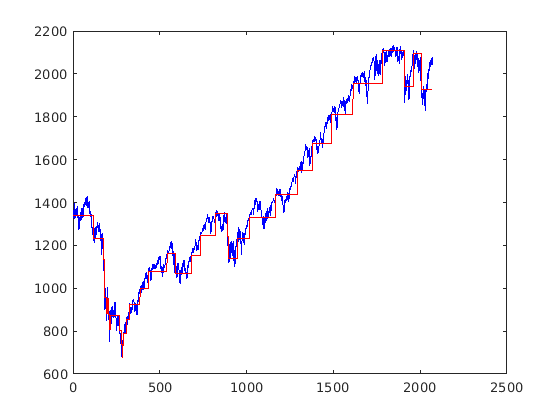
\includegraphics[width=0.6\textwidth]{DiscreteDynamics.png}
\end{figure}

\subsection{event-driven dynamic}
Si considera la seguente event-driven dynamics per il risky asset (k indica il numero di trade)
\begin{equation}
  S_{k+1} = S_{k} (1 + J\Delta \widetilde{N}_{k+1})
\end{equation}
con 
$\Delta \widetilde{N}_{k+1} \sim f_{\Delta \widetilde{N}_{k+1}}$ e

\[
f_{\widetilde{N}_{k+1}}(y) = 
\begin{cases}
p & \text{se} \quad y = 1 \\
1 - p & \text{se} \quad y = -1 
\end{cases}
\]

A questo punto è possibile scrivere la dinamica del valore di portfolio:
\paragraph{dinamica 1} 
\begin{equation} \label{eq:dinamica1}
x_{k+1} = x_k\Big(e^{r \tau} + u^{S}_k J \Delta \widetilde{N}_{k+1}  \Big)
\end{equation}
in cui 
\begin{itemize}
	\item $u^{S}_k$ = peso risky asset, $u^{S}_k \in [-1,1]$
	\item peso risk-free asset costantemente 1 (?)
	\item $r$ = rendimento risk-free asset
	\item $\tau$ =  v.a. che indica il $k+1$-esimo holding time
\end{itemize}

Per poter usare l'algoritmo ODAA è necessario trovare la densità della v.a. in (\ref{eq:dinamica1}). Si trova quindi che 
\begin{equation}
f_{x_{k+1}}(z) = 
\begin{cases}
0 & \text{se} \quad z < x - \xi\\
(1-p)(\frac{\lambda}{r x})\Big(\frac{z+\xi}{x}\Big)^{-(\frac{\lambda+r}{r})} & \text{se} \quad x-\xi \leq z < x + \xi \\
(1-p)(\frac{\lambda}{r x})\Big(\frac{z+\xi}{x}\Big)^{-(\frac{\lambda+r}{r})} + p(\frac{\lambda}{r x})\Big(\frac{z-\xi}{x}\Big)^{-(\frac{\lambda+r}{r})} & \text{se} \quad z \geq x + \xi
\end{cases}
\end{equation}
con $ \xi = xJu^S$

\begin{remark}
	$f_{x_{k+1}} \notin C^0(\mathbb{R})$.Infatti  $z_1 = x - \xi$ e $z_2 = x + \xi$ sono punti di salto
\end{remark}

\paragraph{dinamica alternativa}
In generale la dinamica event-driven per il valore del portfolio è la seguente:
\begin{equation}
	x_{k+1} = x_k\Big( 1 + u^C_k w^C_{k+1} + u^S_k w^S_{k+1}\Big)
\end{equation}
con 
\begin{itemize}
	\item $w^C_{k+1}$ = rendimento cash nel periodo $[t_k,t_{k+1}]$
	\item $w^S_{k+1}$ = rendimento equity nel periodo $[t_k,t_{k+1}]$
\end{itemize}

\vspace*{0.5cm}
\begin{remark}
	l'intervallo $[t_k,t_{k+1}]$ \textbf{non} è deterministico, la sua lunghezza è data dalla variabile aleatoria $\tau_{k+1} \sim \exp(\lambda)$
\end{remark}
\vspace*{0.5cm}
Si vuole trovare quindi un'espressione per i rendimenti dei due asset in funzione di $\tau$ e $\Delta \widetilde{N}_{k+1}$:
\[
\frac{S_{t_{k+1}} - S_{t_{k}}}{S_{t_{k}}} := w^S_{k+1} = J\Delta \widetilde{N}_{k+1} \quad \implies \quad \boxed{w^S_{k+1} = J\Delta \widetilde{N}_{k+1}} 
\]

Per quanto riguarda il risk-free asset, ricordando che $[t_k,t_{k+1}]$ ha lunghezza $\tau$ e $C_{k+1} = C_k\big(1 + w^C_{k+1} \big)$ si ha

\[
C_{k+1} = C_k \Big(1 + r_y\Big)^{\tau} = C_k\exp(r_{\infty}\tau) \quad \implies
\]
\[
\implies \boxed{w^C_{k+1} = \exp(r_{\infty}\tau) - 1 }
\]
avendo indicato con $r_y$ e $r_{\infty}$ il tasso di rendimento del cash composto annualmente e continuamente rispettivamente (entrambi supposti costanti). Per motivi di trattabilità modellistica si suppone il cash evolvere in capitalizzazione esponenziale (composta continuamente) e quindi dai dati si vorrà stimare $ r_{\infty}$.

Si può quindi ricavare la dinamica per il valore di portfolio
\begin{align*}
x_{k+1} & = x_k\Big( 1 + u^C_k w^C_{k+1} + u^S_k w^S_{k+1}\Big)\\
& = x_k\Big(1 + u^C_{k+1} \big(\exp({r\tau}) -1\big) + u^S_{k+1}J\Delta \widetilde{N}_{k+1}\Big)\\
& = x_k \Big(\underbrace{1 - u^C_{k+1}}_{u^S_k} + u^C_{k+1} \exp({r\tau}) +  u^S_{k+1}J\Delta \widetilde{N}_{k+1}\Big) \\
& = x_k \Big(u^C_k\exp({r\tau}) +  u^S_{k+1}(1 + J\Delta \widetilde{N}_{k+1})\Big)
\end{align*}

La densità della v.a. valore di portfolio in questo caso è la seguente
\begin{equation}
f_{x_{k+1}}(z) = 
\begin{cases}
0 & \text{se} \quad z < x u^C - \xi(1-J)\\
(1-p)(\frac{\lambda}{r xu^C})\Big(\frac{z-\xi(1-J)}{xu^C}\Big)^{-(\frac{\lambda+r}{r})} & \text{se} \quad x u^C - \xi(1-J) \leq z < x u^C - \xi(1+J) \\
(1-p)(\frac{\lambda}{r xu^C})\Big(\frac{z-\xi(1-J)}{x}\Big)^{-(\frac{\lambda+r}{r})}+\\ + p(\frac{\lambda}{r xu^C})\Big(\frac{z-\xi(1+J)}{x}\Big)^{-(\frac{\lambda+r}{r})} & \text{se} \quad z \geq x u^C - \xi(1+J)
\end{cases}
\end{equation}
con $\xi = xu^S = x(1-u^C)$

Si riporta infine il grafico della densità di $x_{k+1}$ per diversi valori di $u^C$ (che sarà la variabile rispetto alla quale ottimizzare nell'algoritmo ODAA) e $x = 1.1$, $J = 8\%$ , $r = 2\%$ e $\lambda = 4.41$
\begin{figure}[H]
	\caption{density different $u^C$ (peso cash)}
	\centering
	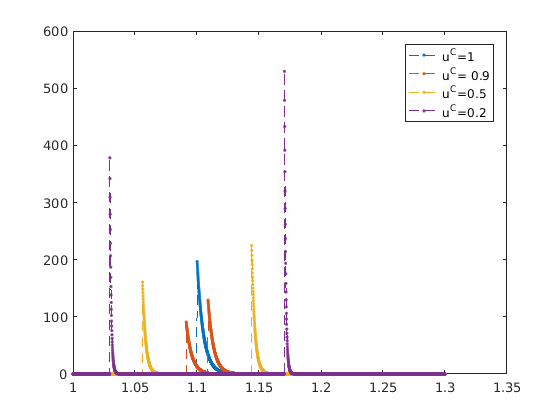
\includegraphics[width=\textwidth]{ptfDensity.png}
\end{figure}

\section{Calibration}
Si devono stimare i parametri $\lambda$ e $p$ per la densità discreta $f_{\Delta N_{k+1}}$.Si utilizza il metodo della massima verosimiglianza.

Da una timeseries del prezzo dell'equity si ricava un campione della v.a. $\Delta N_{k+1}$. Si suppone quindi di avere una realizzazione $\mathbf{y} = \{y_1,y_2,\ldots,y_n\}$, notare che $ y_i \in \{1,-1,0\}, \forall i$. 

La likelihood function si scrive

\begin{equation}
\begin{split}
L(\lambda,p;\mathbf{y}) & = \prod_{i=1}^{n}f(y_i;\lambda,p)\\
& =\Big(\prod_{y_i = 0}\exp(-\lambda\Delta t) \Big)
\Big(\prod_{y_i=1}\big(1-\exp(-\lambda\Delta t) \big)p \Big)
\Big(\prod_{y_i=-1}\big(1-\exp(-\lambda\Delta t)\big)(1-p) \Big)\\
& = \Big(\exp(-\lambda\Delta t) \Big)^\alpha
\Big(\big(1-\exp(-\lambda\Delta t) \big)p \Big)^\beta
\Big(\big(1-\exp(-\lambda\Delta t)\big)(1-p) \Big)^\gamma
\end{split}
\end{equation}

con 
\[ \alpha =  \#\{y_i = 0\}\]
\[ \beta =  \#\{y_i = 1\}\]
\[ \gamma =  \#\{y_i = -1\}\]

Quindi \[
\mathbf{\theta^{\star}} = \arg\max_{(\theta,p) \in \Theta} \log\Big( L(\lambda,p;\mathbf{y})\Big)
\]

\section{Vincolo V@R}
Per imporre un vincolo sulla rischiosità del portfolio occorre calcolare la varianza della v.a.
\begin{equation}
\frac{x_{k+1}-x_k}{x_k} := w_{k+1} = u^C\big(\exp(r \tau)-1\big) + u^S J\Delta \widetilde{N}_{k+1} 
\end{equation}

Si trova che se $ \lambda > 2 r$ 

\begin{equation}
Var[w_{k+1}] = (u^C)^2\frac{\lambda r^2}{(\lambda-2r)(\lambda-r)^2} + 4(u^S J)^2p(1-p)
\end{equation}

Siccome il periodo su cui calcolare il V@R non è deterministico, lo si calcola sul valore atteso di $\tau$. Si può quindi imporre il vincolo
\[
Var[w_{k+1}] \leq \sigma^2_{max}
\]
dove
\[
V@R^{\mathbb{E}[\tau]}_{1-\alpha} = \sqrt{\mathbb{E}[\tau]}V@R^m_{1-\alpha} = \frac{1}{\lambda}V@R^m_{1-\alpha} =  z_{1-\alpha}\sigma_{max} \quad \implies
\]

\[
\implies \qquad \boxed{\sigma_{max} = \frac{V@R^m_{1-\alpha}}{\lambda z_{1-\alpha}}}
\]

\section{Risultati numerici}
$N=10$, $\theta=7\%$, $X_N= [(1+\theta)^2,\infty)$, $r= 5.5\%$, $\lambda = 3.4$, $p = 0.7143$, $J=7\%$, $p^{\star}=$, $p_{MC} = $

\centering
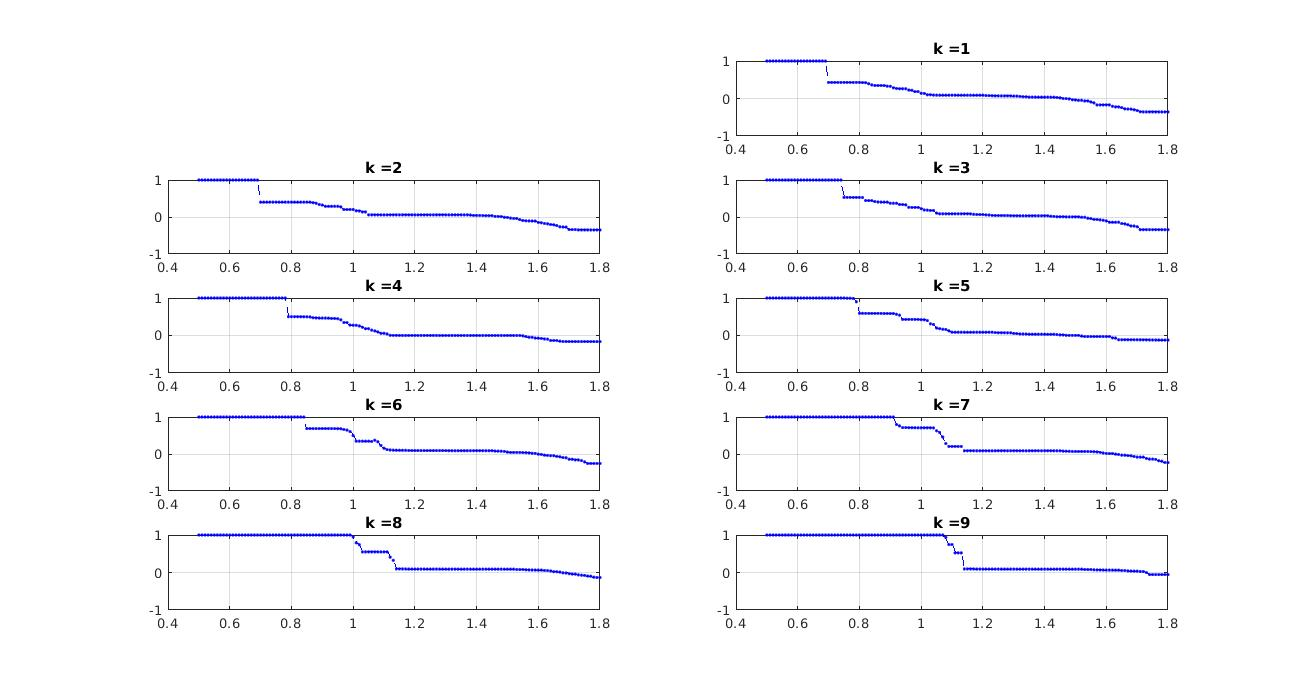
\includegraphics[width=\textwidth,height=0.7\textheight]{maps.jpg}


\end{document}
